% Template for Elsevier CRC journal article
% version 1.2 dated 09 May 2011

% This file (c) 2009-2011 Elsevier Ltd.  Modifications may be freely made,
% provided the edited file is saved under a different name

% This file contains modifications for Procedia Computer Science

% Changes since version 1.1
% - added "procedia" option compliant with ecrc.sty version 1.2a
%   (makes the layout approximately the same as the Word CRC template)
% - added example for generating copyright line in abstract

%-----------------------------------------------------------------------------------

%% This template uses the elsarticle.cls document class and the extension package ecrc.sty
%% For full documentation on usage of elsarticle.cls, consult the documentation "elsdoc.pdf"
%% Further resources available at http://www.elsevier.com/latex

%-----------------------------------------------------------------------------------

%%%%%%%%%%%%%%%%%%%%%%%%%%%%%%%%%%%%%%%%%%%%%%%%%%%%%%%%%%%%%%
%%%%%%%%%%%%%%%%%%%%%%%%%%%%%%%%%%%%%%%%%%%%%%%%%%%%%%%%%%%%%%
%%                                                          %%
%% Important note on usage                                  %%
%% -----------------------                                  %%
%% This file should normally be compiled with PDFLaTeX      %%
%% Using standard LaTeX should work but may produce clashes %%
%%                                                          %%
%%%%%%%%%%%%%%%%%%%%%%%%%%%%%%%%%%%%%%%%%%%%%%%%%%%%%%%%%%%%%%
%%%%%%%%%%%%%%%%%%%%%%%%%%%%%%%%%%%%%%%%%%%%%%%%%%%%%%%%%%%%%%

%% The '3p' and 'times' class options of elsarticle are used for Elsevier CRC
%% The 'procedia' option causes ecrc to approximate to the Word template
\documentclass[3p,times,procedia]{elsarticle}
\flushbottom

%% The `ecrc' package must be called to make the CRC functionality available
\usepackage{ecrc}
\usepackage[bookmarks=false]{hyperref}
    \hypersetup{colorlinks,
      linkcolor=blue,
      citecolor=blue,
      urlcolor=blue}
\usepackage{amsmath}


%% The ecrc package defines commands needed for running heads and logos.
%% For running heads, you can set the journal name, the volume, the starting page and the authors

%% set the volume if you know. Otherwise `00'
\volume{00}

%% set the starting page if not 1
\firstpage{1}

%% Give the name of the journal
\journalname{Procedia Computer Science}

%% Give the author list to appear in the running head
%% Example \runauth{C.V. Radhakrishnan et al.}
\runauth{Beirami et al}

%% The choice of journal logo is determined by the \jid and \jnltitlelogo commands.
%% A user-supplied logo with the name <\jid>logo.pdf will be inserted if present.
%% e.g. if \jid{yspmi} the system will look for a file yspmilogo.pdf
%% Otherwise the content of \jnltitlelogo will be set between horizontal lines as a default logo

%% Give the abbreviation of the Journal.
\jid{procs}

%% Give a short journal name for the dummy logo (if needed)
%\jnltitlelogo{Computer Science}

%% Hereafter the template follows `elsarticle'.
%% For more details see the existing template files elsarticle-template-harv.tex and elsarticle-template-num.tex.

%% Elsevier CRC generally uses a numbered reference style
%% For this, the conventions of elsarticle-template-num.tex should be followed (included below)
%% If using BibTeX, use the style file elsarticle-num.bst

%% End of ecrc-specific commands
%%%%%%%%%%%%%%%%%%%%%%%%%%%%%%%%%%%%%%%%%%%%%%%%%%%%%%%%%%%%%%%%%%%%%%%%%%

%% The amssymb package provides various useful mathematical symbols

\usepackage{amssymb}
%% The amsthm package provides extended theorem environments
\usepackage{amsthm}
\usepackage{subfig}

\newtheorem{definition}{Definition}
\newtheorem{theorem}{Theorem}

%% The lineno packages adds line numbers. Start line numbering with
%% \begin{linenumbers}, end it with \end{linenumbers}. Or switch it on
%% for the whole article with \linenumbers after \end{frontmatter}.
%% \usepackage{lineno}

%% natbib.sty is loaded by default. However, natbib options can be
%% provided with \biboptions{...} command. Following options are
%% valid:

%%   round  -  round parentheses are used (default)
%%   square -  square brackets are used   [option]
%%   curly  -  curly braces are used      {option}
%%   angle  -  angle brackets are used    <option>
%%   semicolon  -  multiple citations separated by semi-colon
%%   colon  - same as semicolon, an earlier confusion
%%   comma  -  separated by comma
%%   numbers-  selects numerical citations
%%   super  -  numerical citations as superscripts
%%   sort   -  sorts multiple citations according to order in ref. list
%%   sort&compress   -  like sort, but also compresses numerical citations
%%   compress - compresses without sorting
%%
%% \biboptions{authoryear}

% \biboptions{}

% if you have landscape tables
\usepackage[figuresright]{rotating}
%\usepackage{harvard}
% put your own definitions here:x
%   \newcommand{\cZ}{\cal{Z}}
%   \newtheorem{def}{Definition}[section]
%   ...

% add words to TeX's hyphenation exception list
%\hyphenation{author another created financial paper re-commend-ed Post-Script}

% declarations for front matter


\begin{document}
\begin{frontmatter}

%% Title, authors and addresses

%% use the tnoteref command within \title for footnotes;
%% use the tnotetext command for the associated footnote;
%% use the fnref command within \author or \address for footnotes;
%% use the fntext command for the associated footnote;
%% use the corref command within \author for corresponding author footnotes;
%% use the cortext command for the associated footnote;
%% use the ead command for the email address,
%% and the form \ead[url] for the home page:
%%
%% \title{Title\tnoteref{label1}}
%% \tnotetext[label1]{}
%% \author{Name\corref{cor1}\fnref{label2}}
%% \ead{email address}
%% \ead[url]{home page}
%% \fntext[label2]{}
%% \cortext[cor1]{}
%% \address{Address\fnref{label3}}
%% \fntext[label3]{}

\dochead{The 16th International Conference on Mobile Systems and Pervasive Computing (MobiSPC) \\ August 19-21, 2019, Halifax, Canada}%
%% Use \dochead if there is an article header, e.g. \dochead{Short communication}
%% \dochead can also be used to include a conference title, if directed by the editors
%% e.g. \dochead{17th International Conference on Dynamical Processes in Excited States of Solids}

    \title{Trusted relational databases with blockchain: design and optimization}

%% use optional labels to link authors explicitly to addresses:
%% \author[label1,label2]{<author name>}
%% \address[label1]{<address>}
%% \address[label2]{<address>}

\author[a]{Amin Beirami}
\author[b]{Ying Zhu}
\author[a]{Ken Pu}

\address[a]{Faculty of Science, UOIT, Oshawa, ON, Canada}
\address[b]{Faculty of Business and IT, UOIT, Oshawa, ON, Canada}

\begin{abstract}
    With the emergence of large scale data collection from Internet of Things
    and mobile computing devices, the notion of trust is becoming an increasing
    important aspects of the next generation of high performant data processing
    systems. We propose a blockchain enabled relational data storage system that
    supports immutable transactions and temporal snapshots.  
    To support large query workloads, we further proposed an optimization
    algorithm that determines the best temporal snapshots to minimize the total
    time cost of answering the given query workload.
\end{abstract}

\begin{keyword}
    trusted database; blockchain; query answering; optimization
\end{keyword}


\end{frontmatter}

\correspondingauthor[*]{Corresponding author. Tel.: +1-905-721-8668}
\email{ken.pu@uoit.ca}

%%
%% Start line numbering here if you want
%%
% \linenumbers

%% main text

%\enlargethispage{-7mm}

\section{Introduction}

In this paper, we study the problem of implementing a trusted relational
database system to support immutable and auditable transactions, and efficient
processing of large numbers of analytical queries.

\subsection{Motivation}

Consider a relational database
used to store purchase orders of various customers and suppliers.  Over time,
customers and suppliers may update the database: insert new orders, 
make modifications to previous ones, or delete existing ones.  Trust is an
exceedingly important aspect of electronic data management. The system must
maintain the provenance of all database transactions in scenarios of dispute.
For example, a customer $C_1$ may claim that an order has been cancelled {\em
before} an agreed deadline, but the
supplier $S_2$ may dispute the time of cancellation.  There are many such
scenarios in practice.
When such disagreements over the history
of the database arise, we would like to have an audit process for which the
finding is {\em indisputable} and hence {\em trusted} by all parties.

We would like to design a trusted relational database system built on existing
and mature technology (such as modern standard RDBMS\footnote{We use Postgresql
for our implementation.}) to store the transactions in such a way that the entire history
of the database is tamper proof.  Namely, while we may not be able to prevent
unwanted modifications to the database (e.g., malicious root users 
or accidental hardware failures), {\em any} modification to the data and its history will be
revealed by an audit process.  In other words, we can {\em trust} the
state of the database by verifying that the database is intact and free of tamper.

Equally important to trust, the database must also support efficient evaluation
of analytical queries.  We envision that many users may submit a large number of
queries, which we will refer to as the {\em query workload}, to the database.  Each
query examines the state of the database at a query specific timestamp.  
Each query may be a simple select query, or one that contains complex data
transformations and aggregations.  So another
functional requirement of the trusted database is to support 
query workloads on a large scale.

\subsection{Problem Definition}
\label{sec:problem-def}

\newcommand{\D}{D}
\newcommand{\U}{U}

Let $\D$ be a relational database.  We are interested in the evolution
of the database, hence the database is parameterized by {\em versions}. 
A database state at some version is given by $\D(t)$
where $t$ is a timestamp.  For simplicity, we will assume $t\in\mathbb{N}^+$.
Let $\U$ be the users.  A transaction is a change applied to the database
(addition, deletion and modification of tuples in $\D$), loosely denoted by
$\Delta\D$.  We also denote the updated database after transaction $\Delta D_t$
submitted by user $u\in\U$ as:
$\D(t+1) = \D(t)+(\Delta\D_t, u)$

When the user is understood, we may write
$\D(t+1) = \D(t) + \Delta D_t$

Assuming that the database starts with an empty initial state, $\emptyset$, at
$t=0$, we define the timeline of the database up to some time $t$ as the series
$\mathrm{TL}(t)$ given by:

$ \mathrm{TL}(t) = 
    \left[\begin{array}{c} \emptyset \\ \mathrm{null} \\ 0 \end{array}\right],
    \left[\begin{array}{c} \D_1 \\ u_1 \\ 1 \end{array}\right],
    \left[\begin{array}{c} \D_2 \\ u_2 \\ 2 \end{array}\right]
    \,\dots\,
    \left[\begin{array}{c} \D_{t-1} \\ u_{t-1} \\ t-1 \end{array}\right].
    $

Namely, $\D_i$ is the $i$-th transaction submitted by user $u_i$ at time $t=i$.

We wish to design a system $\mathbf{DB}$ to manage the timeline $\mathrm{TL}$ with
the following properties:

\begin{itemize}
    \item {\bf Timeline retrieval}: for any time $t > 0$, the timeline
        $\mathrm{TL}(t)$ can be completely retrieved from $\mathbf{DB}$.
    \item {\bf Snapshot retrieval}: for any time $t > 0$, the state of the
        database $D$ can be reconstructed from $\mathbf{DB}$.
    \item {\bf Verification}: There exists a function
        $\mathrm{verify}:\mathbf{DB}\mapsto\{\mathrm{true},\mathrm{false}\}$
        that performs the verification of the system such that
        any {\em tampered} version of the system $\mathbf{DB}'\not=\mathbf{DB}$
        will be fail the verification.  We make no assumption regarding access
        control to the storage,
        so the source of tampering may include root level access to
        $\mathbf{DB}$.  Thus, we limit our problem to {\em detection}, not
        prevention of tampering.
    \item {\bf Query Workload}: let $q$ be some query defined on a snapshot
        $D(t_q)$.  We call $t_q$ the query timestamp.  The system $\mathbf{DB}$
        can efficiently evaluate a large number of such queries with different
        query timestamps.  The collection of queries is called the {\em query
        workload}, written $Q = \{q_1, q_2, \dots, q_N\}$.
\end{itemize}

\section{Related Work}

Trustworthiness has received attention in recent years in various areas
including real-time distributed systems \cite{khayat2017trust}, secret
sharing schemes in the cloud \cite{dutta2013privacy}, and utilizing log files
for forensic analysis \cite{sinha2014continuous}.  

Our work focuses on trusted
transactions in an environment where users cannot be trusted, not even users
with root access to the underlying database. The scenario of privileged
malicious users has been discussed by several researchers
\cite{crosby2009tamper-evident,wagner2018detect,wanger2017carving}. The
approaches
used have been network based and data inspection based detection mechanisms for
database tampering.  In contrast, we rely on embedded blockchains, and do not
require deep access to the system level layer (such as filesystem activity or
network traffic inspection).

There have also been work on database level forensic inspection
\cite{fabbri2013select,hauger2014information} using triggers and related database
features.  When running at scale, triggers can be prohibitively expensive.  Our
approach uses efficient ad hoc inspection of the blockchain structures
to determine the integrity of the database.

Query answering using materialized views is a well established field in database
\cite{du2017deepsea,sohrabi2016materialized,shukla1998materialized,aouiche2006clustering}.
The focus has been on views that are defined by general SQL queries.  In our
work, the snapshots are generated by queries in a very specific form, and thus, we
are able to specialize the materialized view selection problem to obtain a
more efficient algorithm for finding the optimal solution.

\section{Design of trusted relational tables}
\label{sec:trusted-db}

We continue with the problem definition in
Section~\ref{sec:problem-def} and describe the design of the verifiable database
management system.  In our design, we embed a blockchain in the relational
tables to support immutable transactions and verification. This section will
describe the technical elements of the embedded blockchain.

\subsection{Users, keys and digital signatures}

\newcommand{\public}{\operatorname{public}}
\newcommand{\private}{\operatorname{private}}
\newcommand{\enc}{\operatorname{enc}}

Let $U$ be a collection of {\em users}.  Each instance in $U$ can be a user in
the conventional sense, or a device such as Internat of Things (IoT) or a mobile
device.  Without loss of generality, we call all such instances {\em users}.  A
user $u\in U$ is uniquely characterized by a pair of public and private keys:
$\public(u)$, $\private(u)$.  The key pairs are typically generated with large
bits (e.g. 4096-bit) using the RSA scheme \cite{cormen2009introduction} to avoid key conflicts
even in the presence of billions of instances in $U$.  

Given arbitrary data $x$, the encoding function 
$\enc: (x,\private(u))\mapsto \Hat{x}$ where $\Hat{x}$ is a lossless encoding
of $x$, commonly known as the ciphertext.  The ciphertext can be decoded using
the encoding function again, but with the public key:
$$ \enc(\Hat{x}, \public(u)) = x $$

To prove authorship of some data $x$ by user $u$, the following digital signing
scheme is used:

\begin{enumerate}
    \item Compute the hash of $x$ by a fixed hash function: $h(x)$.
    \item Compute the ciphertext of $h(x)$: $\mathrm{sig}(x) = \enc(h(x),
        \private(u))$.
    \item Publish the data, the signature and the public key:
        $\left<x, \mathrm{sig}(x), \public(u)\right>$.
        The published data does not leak the private key of the user.
\end{enumerate}

To verify the authenticity of the authorship from the published data:

\begin{enumerate}
    \item Decode the signature:
        $y = \enc(\mathrm{sig}(x), \public(u))$.
    \item Verify that the decoded signature is the hash value of $x$ using the
        fixed hash function $h$:
        $ h(x) \overset{?}{=} y $
\end{enumerate}

\subsection{Blockchain in relational tables}

We propose a scheme to augment each relational table in a database $D$ with
additional attributes to store the transaction timestamp, a new table signature,
a previous table signature,
and the user public key.  We also need an extra bit flag to indicate if the
transaction is a deletion.  In practice, the bit flat for deletion can be padded
to the end of the transaction signature, but for readability, we assume there is
yet another attribute added to the table of the type boolean.

\newcommand{\attr}{\mathrm{attr}}
For each table $T$ in the database $D$ with attributes $\attr(T)$, we assume
that at least one attribute is the row id\footnote{Popular RDBMS such as MySQL
and Postgresql have built {\tt row\_id} to generate row ids.}.
we augument
the table with the additional attributes: $(\mathrm{t}, \mathrm{sig},
\mathrm{sig}', \mathrm{pubkey}, \mathrm{del?})$ as described above.  We denote
the new table with the augmented attributes as $\Hat T$.
Note, we keep track of two signatures: $\mathrm{sig}$ and $\mathrm{sig}'$
corresponding to the signatures of the table {\em after} and {\em before}
the transaction respectively.  This is necessary to ensure the blockchain
integrity \cite{dhillon2017blockchain,wang2018ablockchain}.

\medskip

{\bf Transaction updates}:  \quad Suppose a user $u\in U$ wants to commit a
transaction $\Delta D$.  Then for each table $T$ involved in the transaction,
let $\Delta T$ be the rows affected (added, modified, or removed).  For each
tuple $x\in\Delta T$, we insert into $\Hat T$ the augmented tuple
$\left<x, i, s, s', \public(u), \mathrm{del?}(x)\right>$ where
$i$ is the current transaction timestamp, $s, s'$ the signatures as
described below, $\public(u)$ the public key of the transaction author, and
finally $\mathrm{del?}(x)$ is the boolean flag indicating if $x$ should be
removed.

The signature is computed as:

\begin{itemize}
    \item $s' = x[\mathrm{sig'}]: x[t] = i-1$. This is unique determined as the
        signature of the previous transaction.
    \item $s = \enc(\mathrm{hash}(\Delta T + s'), \private(u))$. This is the
        digital signature of the transaction data {\em and} the previous
        signature.
\end{itemize}

\medskip

{\bf Verification}: \quad Each table-level transaction $\Delta T$ is uniquely
identified by its timestamp $t$.  It is also uniquely identified by its
signature $\mathrm{sig}_t$.  The verification of the transaction is given as:

$$\mathrm{verify}(\Delta T) = \enc(\mathrm{sig}_t, \public(u)) 
    \overset{?}= \mathrm{hash}(\Delta T + \mathrm{sig}_{t-1}) $$

This allows us to verify all the tables $\Hat T$ in the temporal database.  Any
tampering will be detected by the verification function.



\section{Query answering with optimal snapshots}

\begin{figure}[t]
\centering
\subfloat[Exact optimal cost v.s. heuristic approximation using clustering]{
    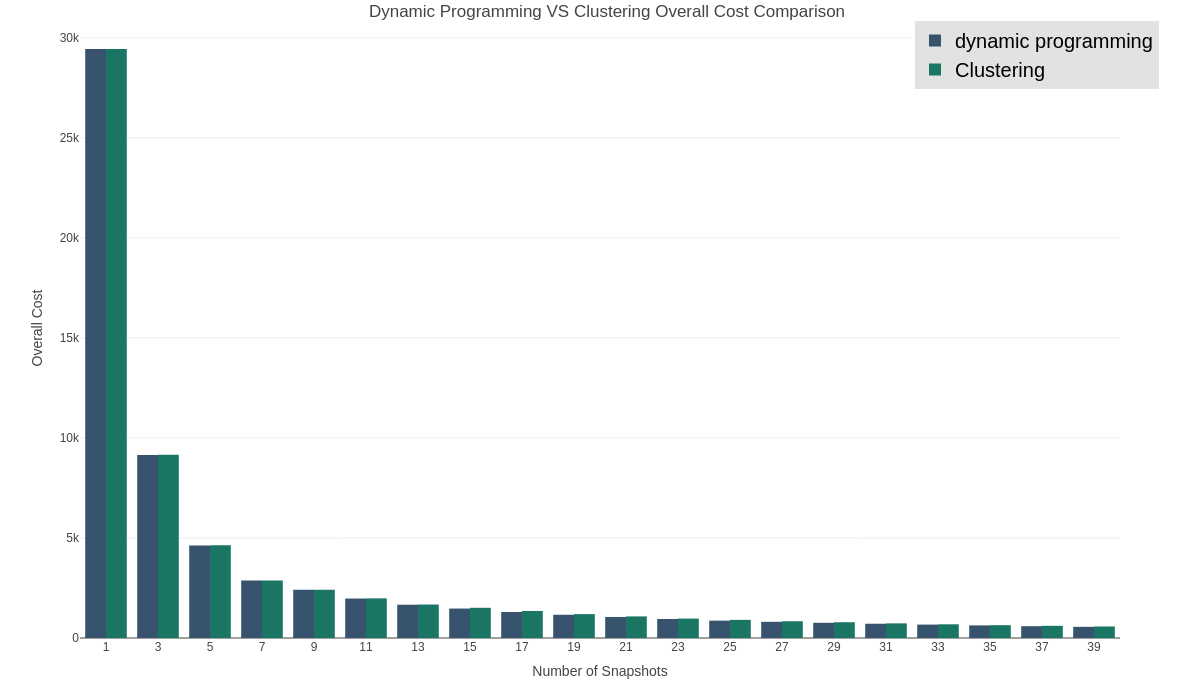
\includegraphics[width=0.45\linewidth]{figs/dynamic_vs_clustering.jpg}
    \label{fig:place-1}
}
\hfill
\subfloat[Approximation quality of 300 iterations vs 5 iterations] {
    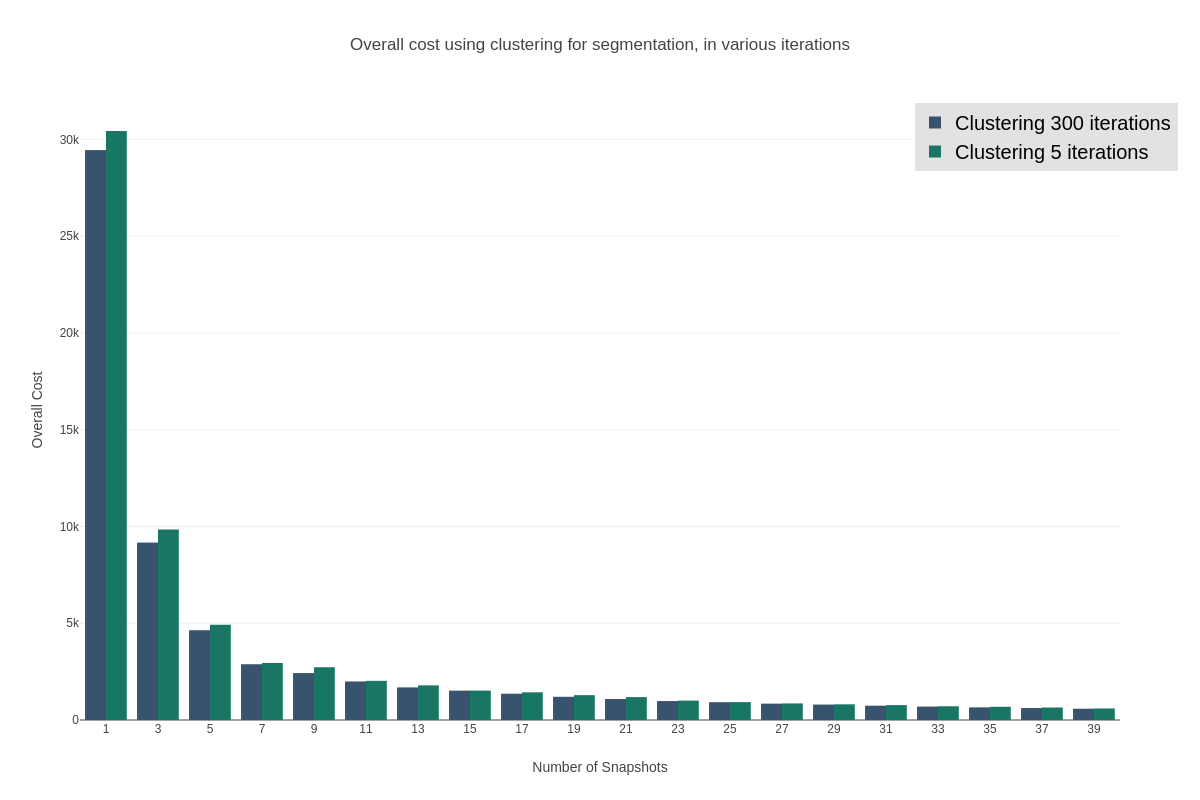
\includegraphics[width=0.45\linewidth]{figs/compare_clustering_iterations.png}
    \label{fig:place-2}
}
    \caption{Quality of the approximate snapshot placements using clustering}
    \label{fig:place}
\end{figure}

\section{Evaluation and experiments}

We have conducted a number of experiments to evaluate the effectiveness of the
proposed algorithms.

A synthetic query workload is generated against a database with over 1
million tuples.  Figure~\ref{fig:query-answer} shows the benefit of having
optimally placed snapshots.  Figure~\ref{fig:query-answer-1} shows the effect of
having just a single snapshot.  One can see that the cost is minimal when the
snapshot is at the median of the query workload of 200.
Figure~\ref{fig:query-answer-2} shows the benefit of having more snapshots
optimally placed.  We see that 40 snapshots, the cost is reduced to less than
1/50 compared to just one snapshot.  Figure~\ref{fig:query-answer-3} shows the
relative performance of different snapshot placement strategies.  We see that
random placement and fixed interval placements are significant worse than the
optimal placement strategy which reduced the cost by over 15 times.

We have compared the runtime performance of the optimal snapshot placement using
dynamic programming and clustering based heuristics.  Figure~\ref{fig:runtime-1}
compares the runtime performance of dynamic programming and clustering with 300
iterations.  One can see that the clustering heuristics scales extremely well
with increasing query workload size.  To further speedup the snapshot placement,
we can reduce to fewer iterations as shown in Figure~\ref{fig:runtime-2}.

The heuristic approach is highly effective in obtaining near optimal snapshot
placements. Figure~\ref{fig:place-1} compares the costs of optimal placement and
approximate placements using 300 iterations.  The increase in the cost is less
than 2%.  Even with just 5 iterations, as shown in Figure~\ref{fig:place-2}, the
resulting approximate is very close to the exact optimal placement.

\section{Conclusion and Future Work}

In this paper, we have presented some results obtained toward optimally
supporting temporal relational queries of databases that store the timelines of
its relational tables.  In order to avoid recomputation of the database states
while making use of the storage space efficiently, our solution is to
materialize $m$ snapshots at well-chosen timestamps.

We have constructed a model to describe the query answering cost, and this cost
model allows us to formulate the $m$-snapshot placement problem as an
optimization problem.  We showed that dynamic programming can be used to solve
the problem {\em exactly}.  Our experimental evaluation demonstrates that our
cost model agrees with relational database systems, and that our snapshot
placements improve query processing significantly.

This is on-going research. As future work, we will be investigating
approximation methods to further speed up the snapshot placement calculuation.
We also wish to investigate maintaining snapshot placement dynamically to cope
with a dynamic query workload.


\bibliographystyle{plain}
\bibliography{src/references}

\end{document}

%%
%% End of file `procs-template.tex'.
